\documentclass[a4paper,11pt]{article}
\usepackage[left=2.5cm, right=2.5cm, top=2cm, bottom=2.5cm]{geometry}
\usepackage{graphicx}
\usepackage{amssymb}
\usepackage{amsmath}

\begin{document}
\title{\LARGE{\textbf{ECEN 202 Lab 3}\\Quiz Night Timer}}
\author{Niels Clayton : 300437590\\ \textbf{Lab Partner: }Billy Robb}
\date{}
\maketitle

\begin{flushleft}
\section*{Introduction}
This lab project tasks us with designing a quiz-night game show timer. Timers are a major component in an array of time limiting games, helping enforce time restrictions on the participants. We will be designing this counter using chips from the 74HCT family.\\The timer should meet the following requirements:\\
\begin{itemize}
\item
Work on a 1Hz clock cycle
\item
Timer should count in one second increments
\item
After 12 seconds, counter will pause and sound a 3 second buzzer
\item
Implement a "Start" button to begin the timer 
\item
Implement a "Answer" button that will pause the timer
\item
Implement a "Reset" button that reset the timer to start
\end{itemize}

\section*{Design Process}
The design of this timer can be broken down into three major components:
\begin{enumerate}
\item
1Hz clock signal generation
\item
MOD-12 ripple counter
\item
three second timer for the buzzer
\end{enumerate}
For each of these components there are many options available to achieve the desired outcome.
\begin{itemize}
\item[-] \textbf{1Hz clock:}\\
For the 1Hz clock there were two possible options. To achieve a frequency of 1Hz you could chose to use a generic 555 Timer chip in astable configuration, which when paired with the correct configuration of resistors and capacitors would produce a 1Hz square wave signal. Alternatively you could directly use the 60Hz frequency of the mains, and after passing it through a MOD-60 counter the output would be a 1Hz frequency square wave.\\Of these options we have decided that we will use the 555 timer timer to generate our clock signal for our circuit. The 555 timer, although less accurate than stepping down mains frequency, allows for easier clock frequency modulation, as well as requiring fewer IC's to be used.
\newpage
\item[-] \textbf{MOD-12 counter:}\\
For the MOD-12 counter there were several available options, with choices of either MOD-16 or MOD-10 (decade) ripple counters available, as well as the ability to concatenate 'J-K' or 'D' flip-flops to build a counter from the ground up. \\ We have chosen to utilise the MOD-10 (decade) ripple counters. This is due to many reasons, Firstly a MOD-10 counter outputs correctly for immediate input into a 7-segment display decoder, however if we were to use the MOD-16 we would need to add external logic to make it a MOD-10. The decade counter therefore allows for the lowest IC count upon implementation.
\item[-] \textbf{Three second counter}\\
With the three second counter there were two options available, we could either take a ripple counter and using external logic convert it to a MOD-3 counter, and then use the same 1Hz clock pulse that drives the main counter to drive the three second buzzer. This would result in a three second period of the buzzer being activated. On the other hand we could use a second 555 timer chip, this time in a monostable configuration, with the correct pairing of resistors and capacitors to produce a 3 second pulse. In our implementation we originally chose to use another counter as a MOD-3 counter in tandem with a D-flip-flop to turn on and of the buzzer for a 3 second period. However after completing the design we found that we had issue with the counter not fully working, and also with the buzzer activation whenever the master reset was activated. Because of this I have re-designed our circuit to now utilise the 555 in monostable mode. This configuration requires the lease IC's and provides the best user experience.
\end{itemize}
\newpage
\section*{Design}
\begin{itemize}
\item[-] \textbf{1Hz clock:}\\
The 1Hz was made using the 555 timer in astable mode as shown in figure 1. This produced a frequency of 1Hz seeing as the frequency of the astable time is given $f = \dfrac{1.44}{(R_{1}+R_{2})C}$
\begin{figure}[ht]
\centering
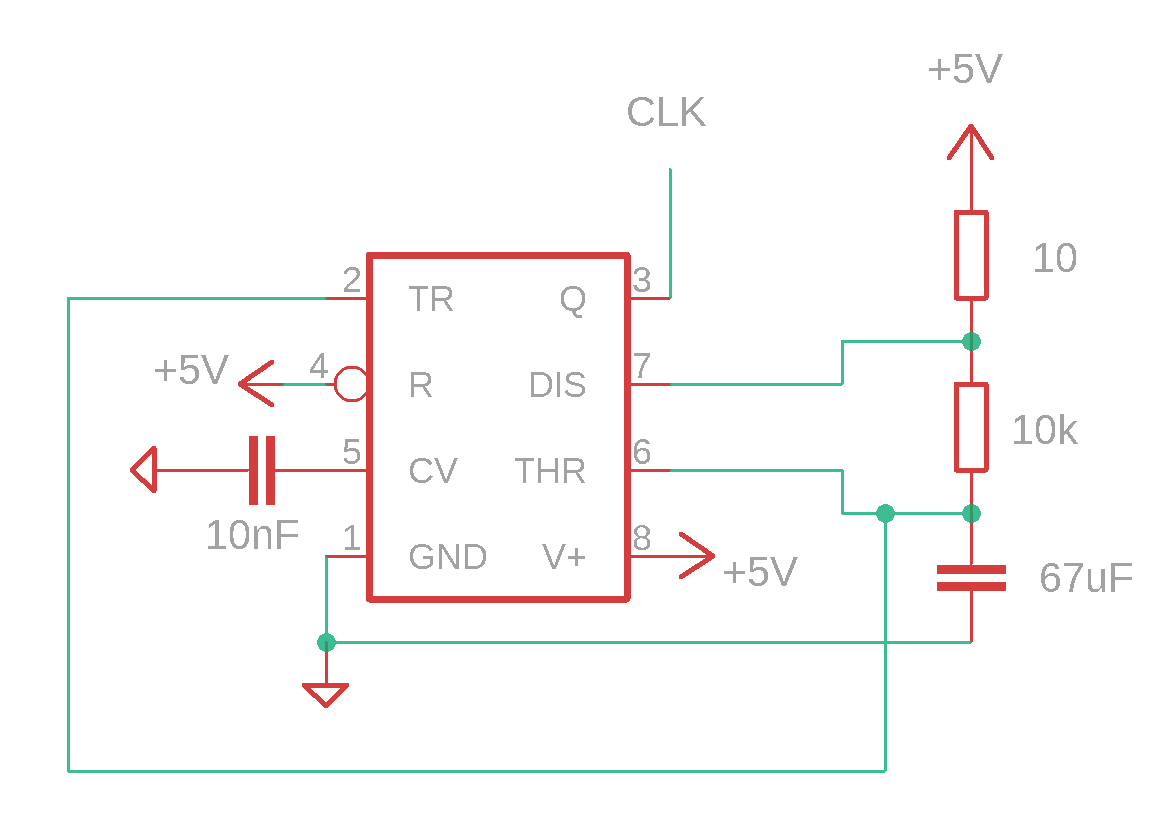
\includegraphics[width=0.7\linewidth]{CLK_timer.png}
\caption{1Hz clock}
\end{figure}
\item[-] \textbf{Three second timer:}\\
The 3 second timer was made using the 555 timer in monostable mode as shown in figure 2. This configuration produces a pulse duration of 3 seconds as soon as the trigger pin(pin 2) is pulled high.\\$Period =1.1\times R\times C$
\begin{figure}[ht]
\centering
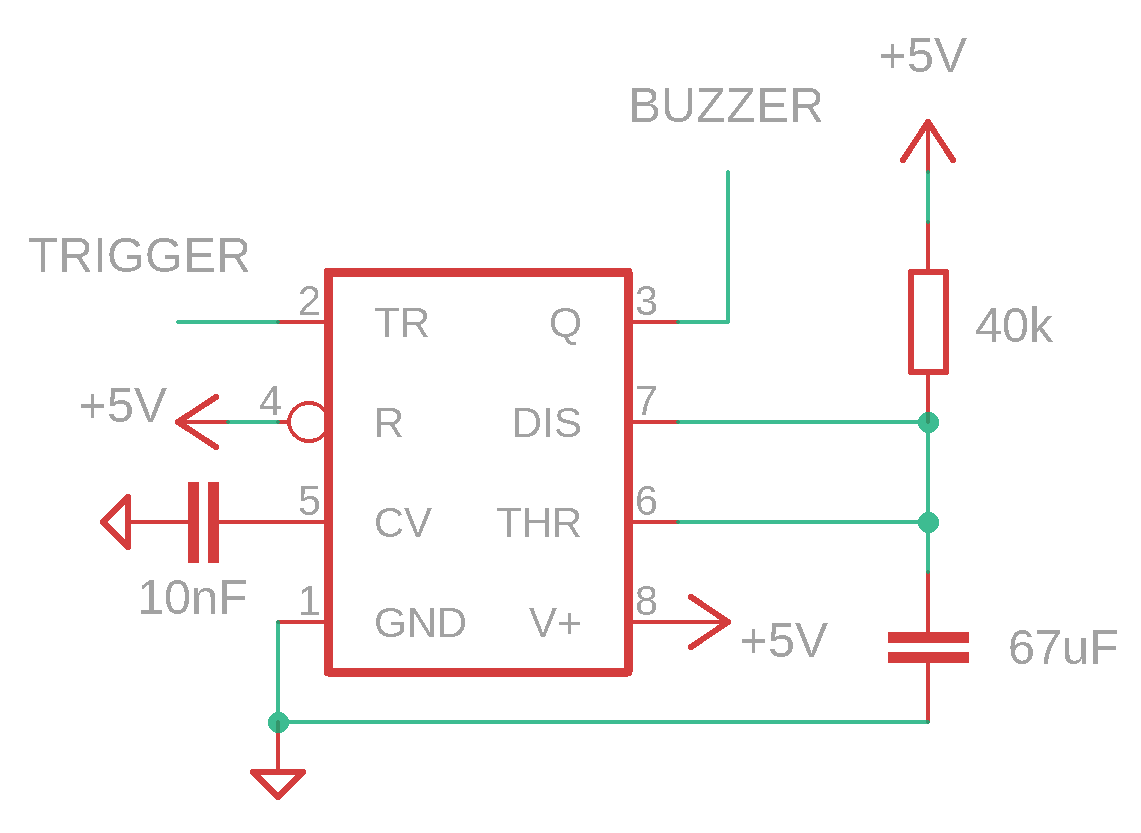
\includegraphics[width=0.7\linewidth]{OneShot_Timer}
\caption{Three second timer}
\end{figure}
\newpage
\item[-] \textbf{MOD-12 counter}\\
The MOD-12 counter is comprised of two MOD-10 counters concatenated, providing a MOD-100 counter. This is then reduced to a MOD-12 counter using external logic. The 'JK' flop-flop is then used along with the user contestant button, and then and with the clock pulse to make it possible to pause the counter at any point, and then resume counting again by toggling the JK. Because of this configuration, upon reaching the 12th clock pulse, or when the contestant button is pushed, the counter will toggle the JK, which will then no longer AND with the clock, and the time will remain paused on the displays.
\begin{figure}[ht]
\centering
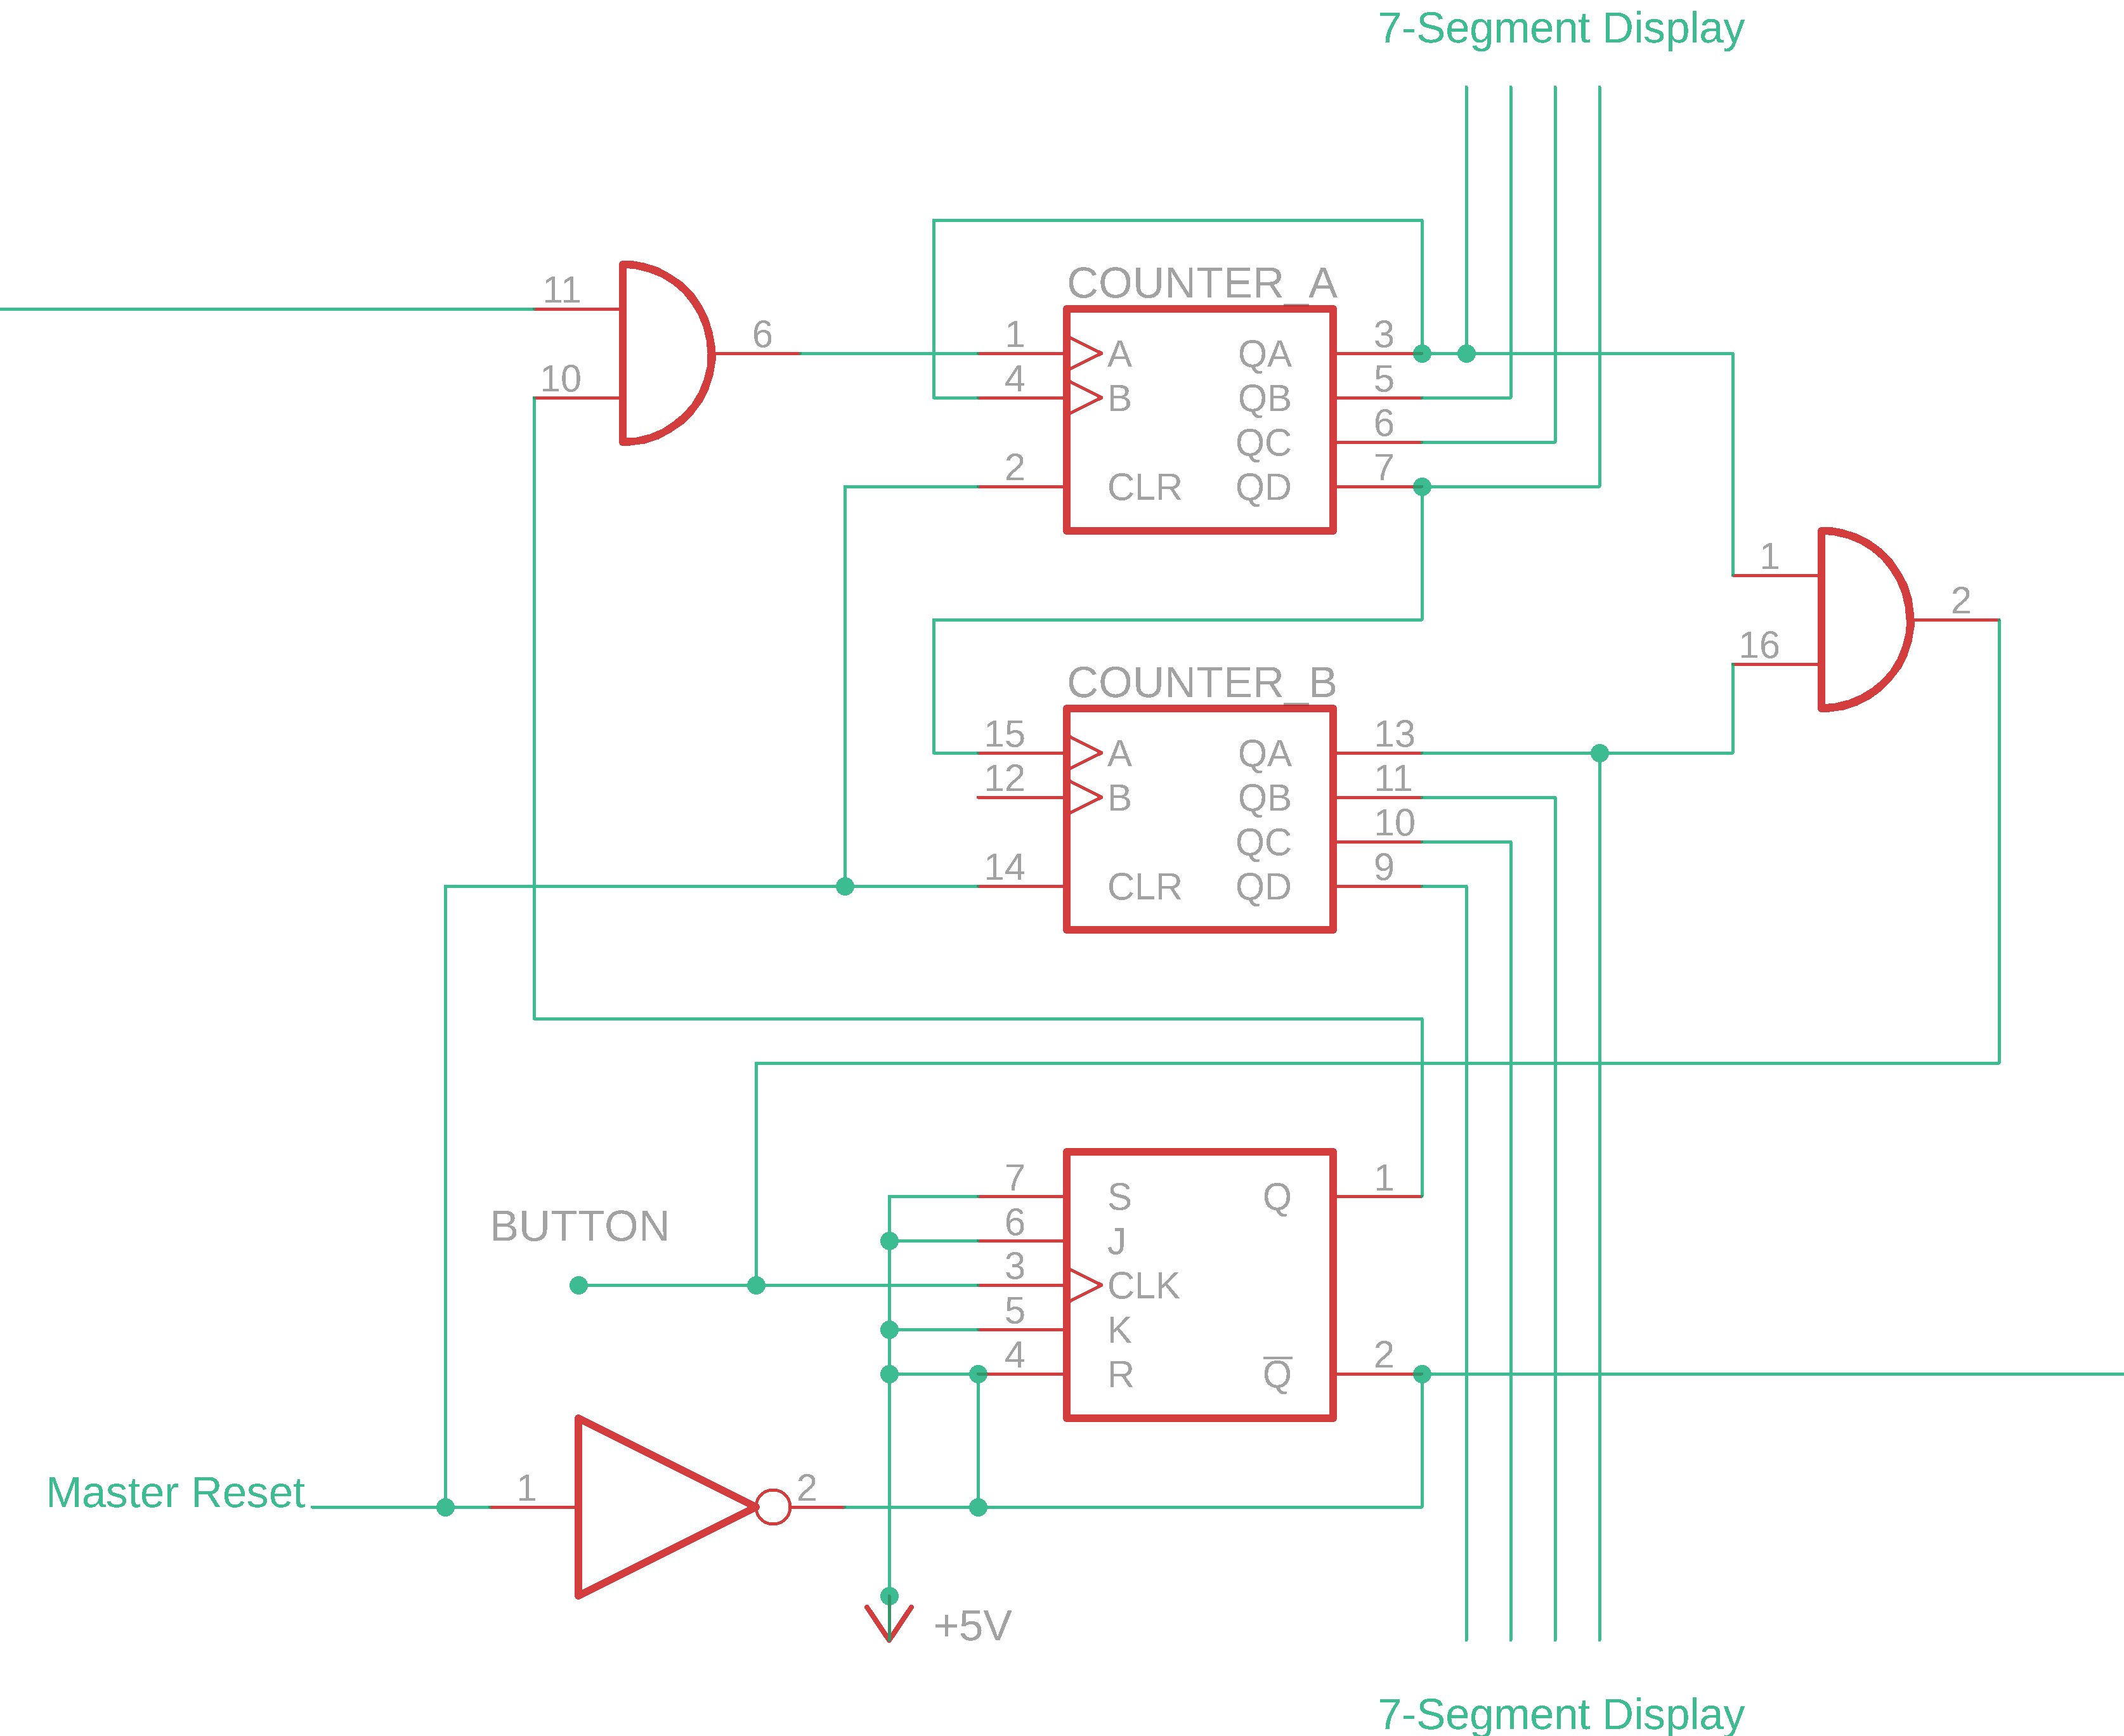
\includegraphics[width =\linewidth]{counter}
\caption{MOD-12 counter}
\end{figure}
\end{itemize}
\newpage
\section*{Testing}
In order to test if this circuit configuration works, we built the circuit during our assigned lab period using the design stations in the lab, and the provided HCT74 series chips. The design stations in our lab have inbuilt 7-segment display drivers, allowing for the removal of those chips from all proposed designs above. However if this design were to be extrapolated and used outside of the lab, these decoders would need to be incorporated onto the design.
\begin{figure}[ht]
\centering
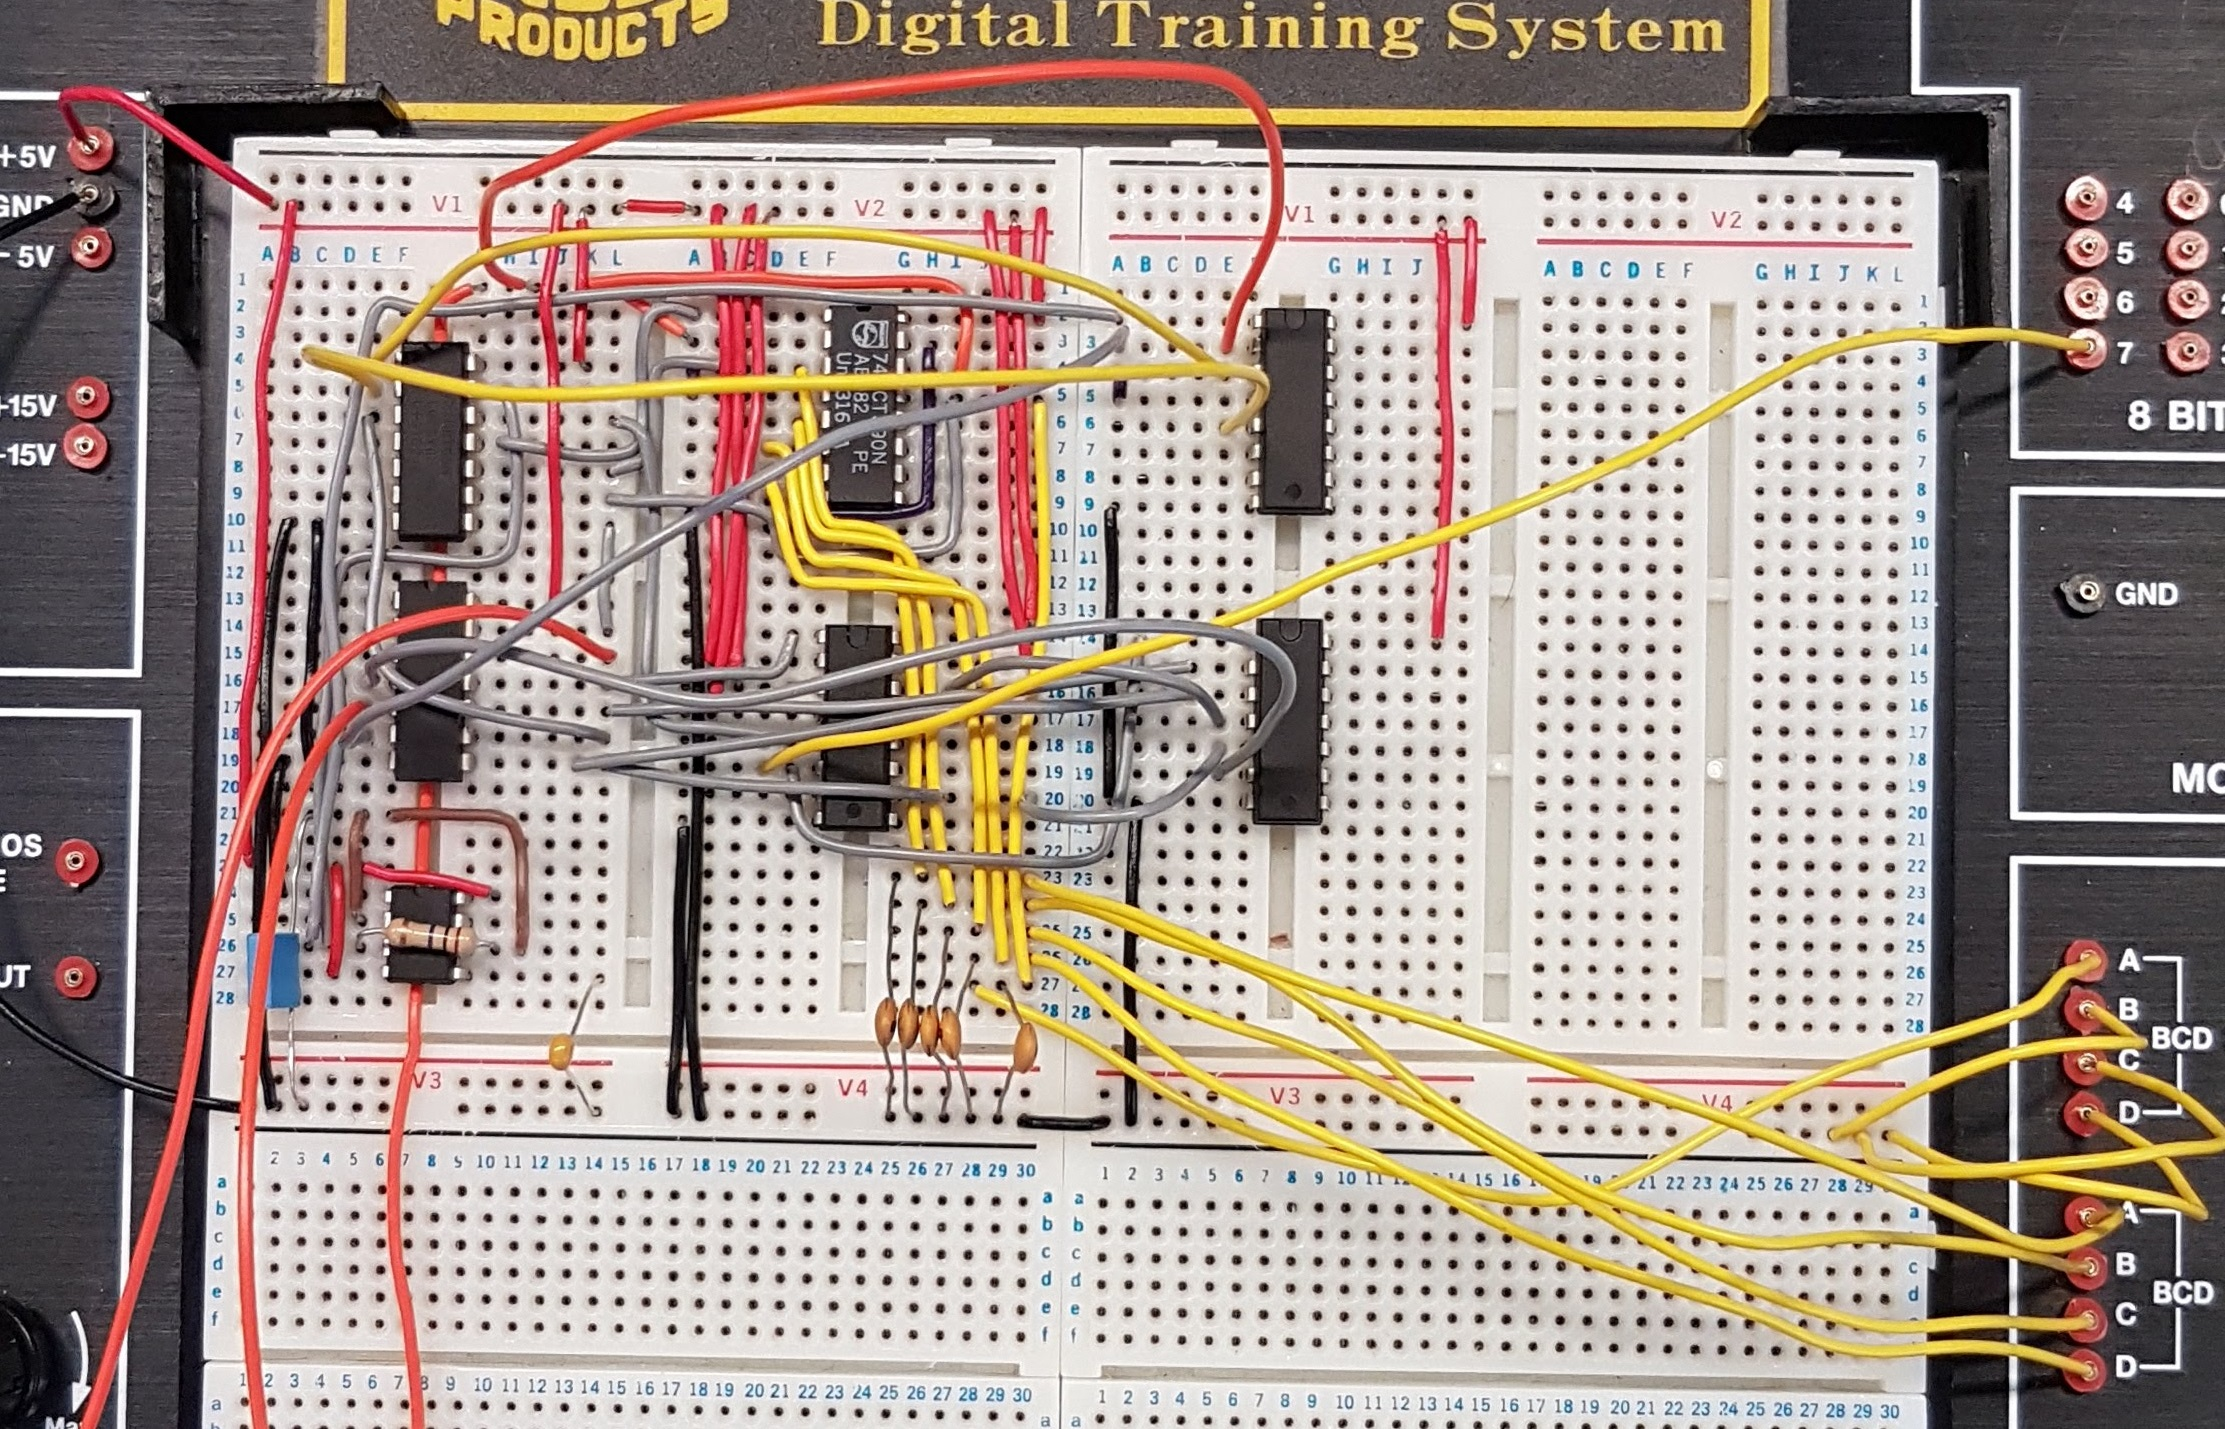
\includegraphics[width =\linewidth]{breadboard_complete_1}
\caption{Test design of circuit}
\end{figure}
When testing we realised that our design for the 3 second counter would be be effective for our purposes, as we were unable to reset the circuit without setting off the buzzer. Because of this if you were to produce a similar circuit it would be recomended to use the 3 second monostable 555 timer shown in figure 2. This used in tandem with a simple edge detection circuit would allow for the 3 second buzzer to be activated without issue.
\newpage
\begin{figure}
\centering
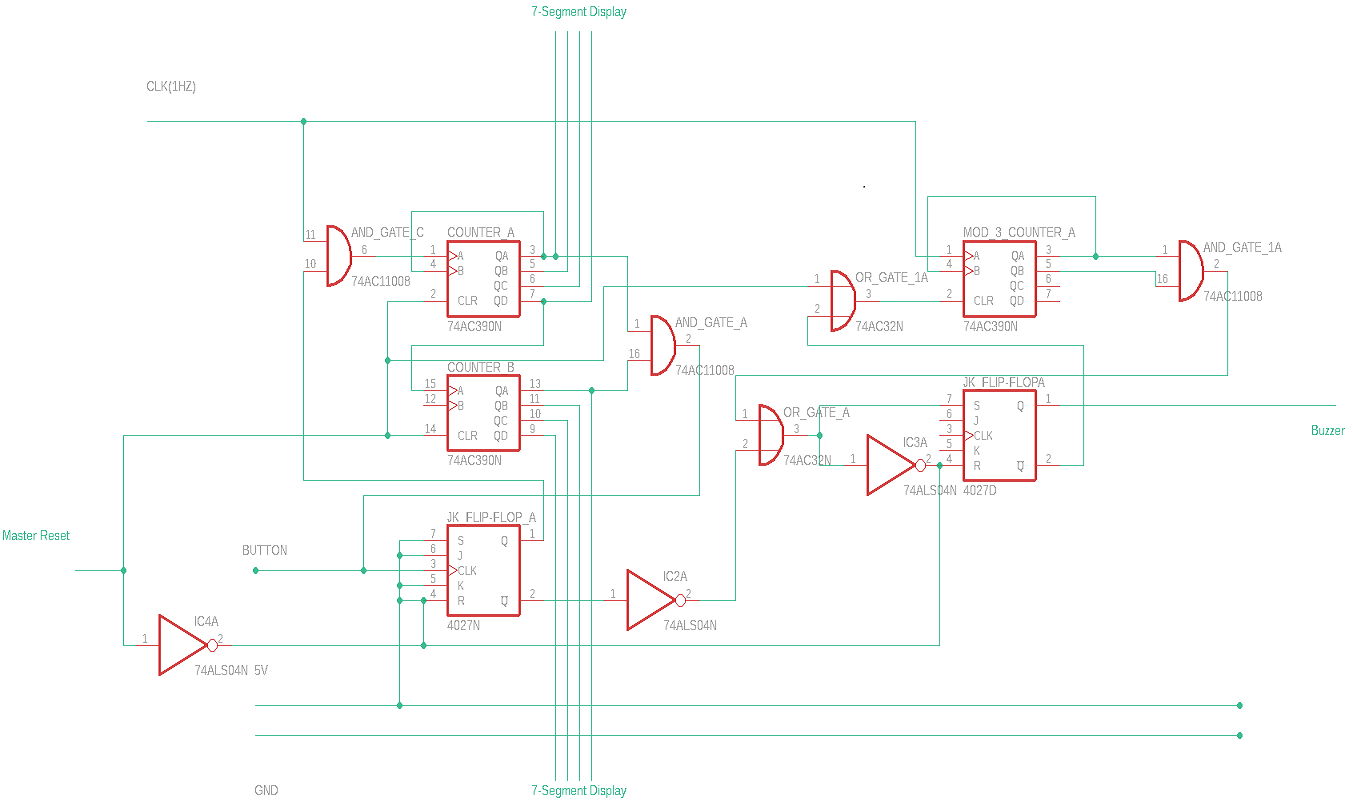
\includegraphics[]{circuit_design_202}
\caption{Original circuit design}
\end{figure}

\begin{figure}[H]
\centering
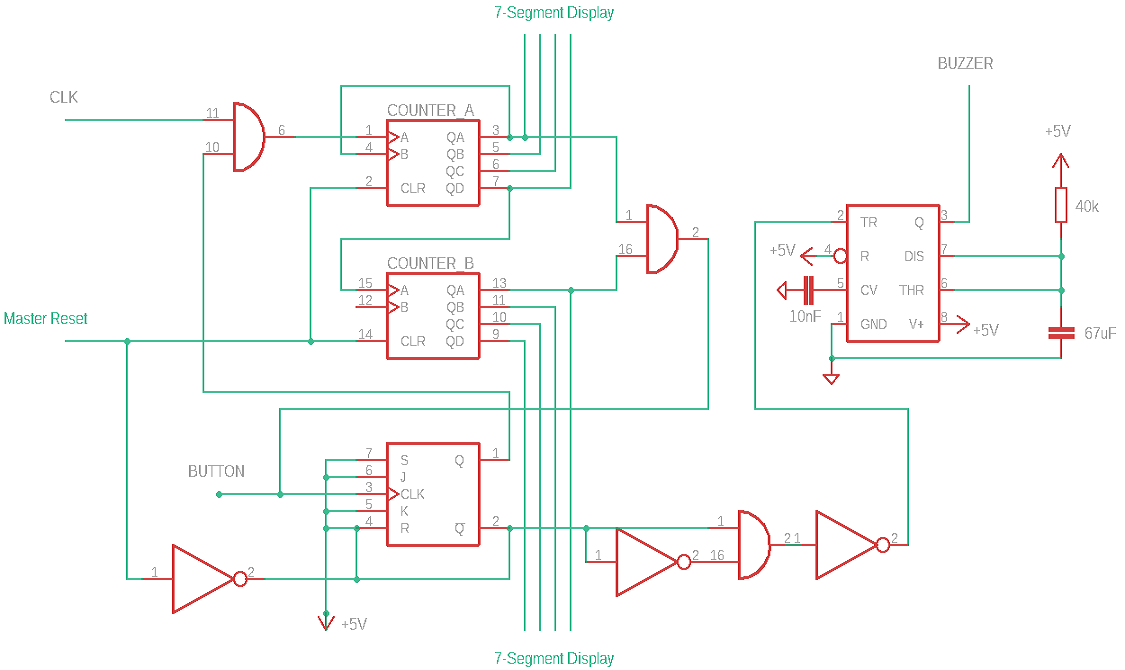
\includegraphics[width = 0.9\linewidth]{Circuit_improved}
\caption{improved circuit design}
\end{figure}
\newpage

\section*{Conclusions}
Overall our design was successful in achieving the 1Hz clock, The 12 second counter, implementing a start, a reset, and a contestant button, however it was unable to successfully implement the three second timer. Because of this we have reviewed the design and improved upon it, making it more simplistic, easy to assemble, reliable, and fit for purpose. \\
Overall this project was thought provoking, and highly enjoyable, the only aspect that was unpleasant was the use of the workstations, at they had very intermittent 7-segment display decoders.
						
\end{flushleft}
\end{document}
